\documentclass[titlepage, 11pt]{article}
\usepackage[a4paper, total={6in, 9.5in}]{geometry}
\usepackage{graphicx}
\usepackage{amsfonts,amssymb}
\usepackage{amsmath}
\usepackage{listings}
\usepackage{booktabs}
\usepackage[T1]{fontenc}
\usepackage{listings}
\usepackage{color}
\usepackage{minted}
\usepackage[colorlinks=true, linkcolor=blue, urlcolor=blue, citecolor=blue, pdfborder={0 0 255}]{hyperref}
\usepackage{colortbl}
\usepackage{url}
\usepackage{xcolor}
\usepackage{caption}
\usepackage{subcaption}
\usepackage{dirtytalk}
\usepackage[semicolon, round]{natbib}
\usepackage[ruled]{algorithm2e}
\captionsetup[table]{skip=10pt}
\renewcommand{\vec}[1]{\mathbf{#1}}
\SetKwComment{Comment}{$\triangleright$\ }{}
 \hypersetup{%
 	colorlinks=true,
 	linkcolor=blue,
 	linkbordercolor={0 0 1}
 }

% \renewcommand\lstlistingname{Algorithm}
% \renewcommand\lstlistlistingname{Algorithms}
% \def\lstlistingautorefname{Alg.}

 \lstdefinestyle{Python}{
 	language        = Python,
 	frame           = lines, 
 	basicstyle      = \footnotesize,
 	keywordstyle    = \color{blue},
 	stringstyle     = \color{green},
 	commentstyle    = \color{red}\ttfamily
 }

% \setlength{\parindent}{0.0in}
% \setlength{\parskip}{0.05in}

\newcommand{\argmin}{\mathop{\mathrm{argmin}}}
\newcommand{\argmax}{\mathop{\mathrm{argmax}}}
\newcommand{\minimize}{\mathop{\mathrm{minimize}}}
\newcommand{\maximize}{\mathop{\mathrm{maximize}}}
\newcommand{\st}{\mathop{\mathrm{subject\,\,to}}}
\newcommand{\dist}{\mathop{\mathrm{dist}}}
\newcommand{\norm}[1]{\left\lVert#1\right\rVert}
\renewcommand{\vec}[1]{\mathbf{#1}}

\def\R{\mathbb{R}}
\def\E{\mathbb{E}}
\def\P{\mathbb{P}}
\def\S{\mathbb{S}}
\def\Cov{\mathrm{Cov}}
\def\Var{\mathrm{Var}}
\def\half{\frac{1}{2}}
\def\quat{\frac{1}{4}}
\def\sign{\mathrm{sign}}
\def\supp{\mathrm{supp}}
\def\th{\mathrm{th}}
\def\tr{\mathrm{tr}}
\def\dim{\mathrm{dim}}
\def\dom{\mathrm{dom}}

\begin{document}
 
\title{
    {EE2703: Simulated Annealing} \\\
    {\vlarge Programming Assignment {\#} 7}\
}
\author{Student's Name, Roll Number\
    : & Annangi Shashank Babu, EE21B021}
\date{\today}     
\maketitle
\setcounter{page}{0}
\tableofcontents
\listoffigures
\listoftables
\newpage
\section{Function Minimisation}
Simulated Annealing is a popular \textbf{optimization} algorithm used to find the global minimum of a given function.
The algorithm uses the concepts of decaying learning rate and randomisations to 
find the optimal solution. 
\\
\\
Simulated Annealing works by deviating from the current point by a random distance (but as temperature decreases we should deviate less from the current point) 
and evaluating the function at that point.The new point becomes the current point if it has a lower function value than the current point. Based on the temperature and learning rate, the algorithm may still accept the new point with a given probability even if it has a greater function value than the existing point. The likelihood of accepting a new point with a higher function value reduces as the temperature rises. 
This procedure continues until the algorithm reaches a maximum number of iterations.
\lstinputlisting[style=Python]{cl.py}
\subsection{Ouptut}
for the function : 
\begin{centre}
    $f(x)  =  x^2 + sin(8*x)$
\end{centre}
\begin{figure}[ht]
    \centering
    \includegraphics[width=0.8\textwidth]{function_minimisation.jpeg}
    \caption{Output for the given function}
    \label{fig:function minimisation jpeg}
\end{figure}
\\
Output of the code : The minimum value occurs at -0.18099753460055526, minimum 
being -0.9597074766558362

\section{Travelling Salesman Problem}
\subsection{Recursion}
The first brute force approach to solve the Travelling salseman problem is to calculate the distance covered for every single path
and findout the minimum travel path, this can be achived from recursion which is of factorial time complexity, with introduction of 
dynamic programming we can reduce to time complexity to exponential.
\lstinputlisting[style=Python]{al.py}
\subsubsection{Output}
The output for the case of 10 cities : 
\begin{figure}[ht]
    \centering
    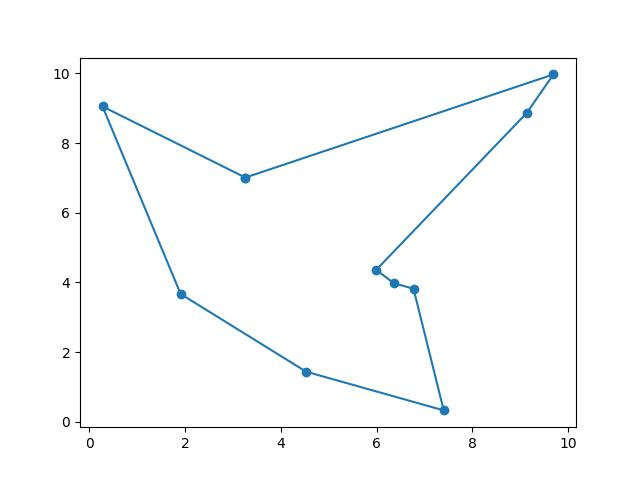
\includegraphics[width=0.8\textwidth]{r_tsp10.jpeg}
    \caption{Ouput using recursion}
    \label{fig:tsp 10 jpeg}
\end{figure}
the order and the total distace of travel are mentioned in the file named \textbf{r out10.txt}.

\subsection{Simulated Annealing}
Now we use the simulated annealing algorithm to solve the travelling salesman problem, the optimisation algoritms come into 
play when the time complexity  of solving a problem is exponential or factorial and definite solution for large inputs cant be found in 
finite time by a modern computer
\begin{itemize}
    \item Choose a random permutation of the cities to visit.
    \item Initially, the temperature is high, allowing the algorithm to accept worse solutions.
    As the temperature decreases, the algorithm becomes more selective and only accepts better solutions.
    \item If the new solution is better than the current solution, accept it as the new current solution.
    If the new solution is worse than the current solution, accept it with a certain probability that depends on the temperature and the difference in cost between the new and current solutions.
    \item After the iterations, return the best solution found, which is the solution with the lowest cost.
\end{itemize}

\lstinputlisting[style=Python]{bl.py}
\subsubsection{Output for 10 cities}
\begin{figure}[ht]
    \centering
    \includegraphics[width=0.8\textwidth]{tsp_10.jpeg}
    \caption{The output for the 10 cities testcase}
    \label{fig:tsp 10 jpeg}
\end{figure}
\\ 
the order and the total distace of travel are mentioned in the file named \textbf{out10.txt}.
\\
\\
\subsubsection{Output for 100 cities}
For the 100 cities case :
\begin{figure}[ht]
    \centering
    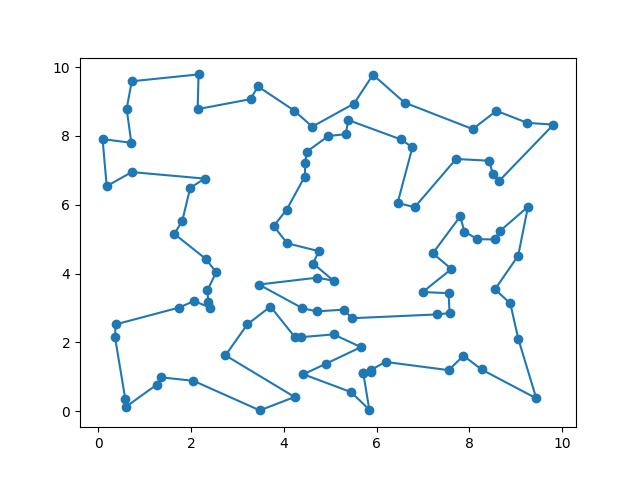
\includegraphics[width=0.8\textwidth]{tsp_100.jpeg}
    \caption{The output for the 100 cities testcase}
    \label{fig:tsp 100 jpeg}
\end{figure}
\\
the order and the total distace of travel are mentioned in the file named \textbf{out100.txt}.

\section{Conclution}

Both parts require a solid understanding of optimization techniques, such as Simulated Annealing and Reccursion, as well as problem-solving skills to apply these techniques to the given problems. The ability to read and parse input files and generate output plots is also necessary.

The hyper-parameters must be tuned properly to get better results, such as selecting a decay rate so that at the end of all
the iterations the temperature is relatively small quantity (around -1e-5 was giving perfect result for above case) and decay rate must
not be too small also which will lead to a rapid decay in temperature and causes to end up in a local minima.
\\
\\
Overall, this assignment tests our knowledge and skills in optimization and problem-solving.


%%%%%%%%%%%%%%%%%%%%%%%%%%%%%%%%%

% Uncomment the lines below to add references using bibtex.
% \bibliographystyle{plainnat}
% \bibliography{references}

\end{document}

